\documentclass[sigconf]{acmart}

\usepackage{listings}
\usepackage{booktabs} % For formal tables
\usepackage{algorithm}
\usepackage{algorithmic}
\usepackage{enumitem}
\usepackage{amsthm}
\setcopyright{rightsretained}

% DOI
\acmDOI{10.475/123_4}

% ISBN
\acmISBN{123-4567-24-567/08/06}

%Conference
\acmConference[WOODSTOCK'97]{ACM Woodstock conference}{July 1997}{El
  Paso, Texas USA} 
\acmYear{1997}
\copyrightyear{2016}

\acmPrice{15.00}

\newtheorem{insight}{Insight}

\begin{document}
\title{Automatic Tuning of SQL-On-Hadoop Engines on Cloud Platforms}

\author{Prasad Deshpande}
\affiliation{%
  \institution{Qubole India}
  \city{Bengaluru}
  \state{Karnataka}
  \country{India}
}
\email{pmd@qubole.com}

\author{Amogh Margoor}
\affiliation{%
  \institution{Qubole India}
  \city{Bengaluru}
  \state{Karnataka}
  \country{India}
}
\email{amoghm@qubole.com}

\author{Rajat Venkatesh}
\affiliation{%
  \institution{Qubole India}
  \city{Bengaluru}
  \state{Karnataka}
  \country{India}
}
\email{rvenkatesh@qubole.com}

% The default list of authors is too long for headers}
\renewcommand{\shortauthors}{P. Deshpande et al.}


\begin{abstract}
More and more companies are running Big Data workloads on cloud platforms. Configuration tuning of data engines continues to be an essential but difficult undertaking. Cloud Platforms provide elasiticity of compute resources through auto-scaling and different machine types. This choice further exacerbates the problem of choosing the best configuration. ETL engineers have to choose the correct machine type as well as \# of machines along with other configuration options.

In this paper, we propose to build a model that optimizes performance and cost. Cost is as important a metric as performance in cloud deployments. The model consists of rules and heuristics to optimize performance. In the next phase, the model considers the available machine types and prices to optimize cost. 

We chose to focus on SQL workloads because SQL or SQL-like languages continue to be the most popular choice of ETL engineers and analysts. We show that very simple models of SQL Data Engines can provide very good recommendations compared to the optimal configuration and these are also better than those chosen by experts. Furthermore, we focus on SQL-on-Hadoop technologies but the principles behind model is generic and can be adopted for any big data engine. 
\end{abstract}

\keywords{Big Data, SQL, Hadoop, Hive, Presto, Spark, Automatic Performance tuning}


\maketitle

\section{Introduction}

With the widespread adoption of cloud technologies, companies of all sizes are choosing to host their compute infrastructure on cloud platforms like AWS, Micrsoft Azure and Google Cloud Platform. 
Many of the best practices from in-house data center administration and tuning are also carried over to the cloud. However, cloud platforms have several unique properties like elasticity, separation of compute and storage, short lived clusters, and availability of different machine types. As big data infrastructure companies have matured, they are building systems that exploit some features of cloud platforms effectively. For example, Qubole provides auto-scaling 
and heterogenous clusters for Apache Hadoop, Apache Spark and PrestoDb systems. 

However, automatic workload tuning and capacity planning have not yet reached the same level of maturity as auto-scaling on cloud platforms. By tuning a workload, we mean determining a good set of configuration parameters and cluster settings for the queries to run efficiently. Organizations need to rely on experts to optimize big data systems for their workloads. However, the 
complexity of big data technologies and workloads combined with the choice provided by the flexibility of cloud platforms makes manual tuning unscalable. 

In this paper, we address the problem of automatically determining good configuration parameters for SQL workloads with the goal of optimizing resource usage and cost. We present two alternatives -- an iterative method based on repeatedly executing queries with different configuration parameters and a model based method that relies on simple rules and insights. Both of these approaches have been proposed in some form in prior works. For example,~\cite{KumarPLPGB16} uses an simultaneous perturbation stochastic approximation (SPSA) based iterative algorithm to discover good configuration parameters. In the model based category, Starfish~\cite{herodotou2011profiling, herodotou2011starfish} was the one of the first systems to develop a comprehensive model for Hadoop map-reduce (MR) based systems. These previous works were directed towards generic workloads running on Hadoop systems, which increases the complexity of the problem due to the large number of possible configuration parameters and factors affecting system performance. This makes the iterative approach too expensive in practice due to large number of iterations. The model based approach, on the other hand, becomes very complex and brittle since they require the model to simulate every aspect of a data engine.

Our experience with customer workloads at Qubole suggests that SQL or SQL-like languages continue to be the most popular choice of ETL engineers and analysts. Thus, we chose to focus on SQL Workloads in our work rather than generic workloads. Since the mechanism of SQL query processing is well understood, we can use that knowledge to identify a smaller subset of configuration parameters that have significant impact on the query processing time and focus on optimizing them. 


We started with an iterative approach applying some more optimizations such as discretization, range reduction and dimension independence to further reduce the search space. Experiments on synthetic and real datasets show that the iterative algorithm was able to reduce resource utilization significantly (upto 80\%) compared to the default (for synthetic workloads) or expert chosen values (for real workloads) in a small number of iterations (usually around 10-15). However, the dollar cost of even the smaller number of iterations makes it practically infeasible.

We then moved to the model based approach that uses rules and heuristics to optimize performance and cost. Rules for performance optimization use data statistics from the catalog or previous runs. We further extended the model for cloud platforms by adding rules that use machine type to factor in the resources available for a workload. The model optimizes cost by computing expected run times for all machine types and choosing the best combination of run time and price per machine. The goal of the model was not to predict the run time exactly, but rather to be able to accurately compare the relative performance of two sets of configuration parameters. The surprising result is that a very simple rule based model is able to provide very good recommendations leading to significant savings in resource usage and cost. In fact, we found that these were often better than those chosen by experts on real customer workloads.

%Another important factor is the focus on SQL Workloads. Prior attempts at model based approach required models to simulate every aspect of a data engine. The advantage is that the approach is generic but the disadvantage is that it is complex and brittle. Prior research and our results show that a simple model is good enough for SQL Workloads. We compare the configuration values generated by the model with those determined by experts. Since experts did not choose optimal parameters, we determined optimal parameters using an iterative approach and compare with it as well.

The rest of the paper is organized as follows. Section~\ref{sec:relatedwork} gives an overview of the related work and Section~\ref{sec:optmethod} defines the objectives of the optimization process. Section~\ref{section:iter} describes the iterative approach and its results on real and synthetic datasets. Section~\ref{sec:insights} presents the insights that feed into developing the model based approach, which is detailed in Section~\ref{sec:modelbased} along with the experimental results. An extension of this approach for cloud platforms is presented in Section~\ref{sec:modelcloud}. We finally conclude in Section~\ref{sec:conclusions}.

\noindent\subsubsection*{Experimental Setup}
Qubole\cite{qubole} provides proprietary versions of Apache Hive\cite{thusoo2009hive}, Apache Spark\cite{zaharia2016apache} and Facebook Presto\cite{presto} to its customers.
All experiments were run on Apache Hive and Apache Spark using Qubole Data Service (QDS) on Amazon Web Services (AWS). 
The models and experiments do not use any proprietary extensions of QDS.  
Due to budget and contract constraints, we have presented results from different customer workloads which consists of different data, queries, engine, cluster and machine configuration.
To ensure consistency, we present results for each approach (iterative, model and cloud model) from a single company using a specific dataset, query set and data engine. 
Results for each approach are self-contained and independent. Moreover the variety of experiments and setup show the versatility of our approach. 

A brief overview of the customers who provided permission to run experiments and their technology stack are:
\begin{enumerate}
	\item[$\bullet$] Customer 1: A large e-commerce company that uses Apache Hive executed on Hadoop2 MR engine to process click stream and product data. 
	\item[$\bullet$] Customer 2: A large travel logistics company that uses Apache Hive executed on Hadoop2 MR engine to process data on demand and usage of its services.
	\item[$\bullet$] Customer 3: A Platform-As-A-Service company that uses Apache Spark to process telemetry data from its platform.
\end{enumerate}

Section~\ref{section:iter} on iterative approach contains experimental results at Customer 1 using Apache Hive on Hadoop 2 MR engine. 
For this reason we also present results of the synthetic workload using Apache Hive on Hadoop 2 MR engine. 
In Section~\ref{sec:insights} and Section~\ref{sec:modelbased} we generate insights and build a model using Apache Spark. 
We ran experiments for model-based approach at both Customer 2 and Customer 3. 
Therefore we modified the model for Apache Hive on Hadoop and present results for both. In Section~\ref{sec:modelcloud} we present results from Customer 3 on Apache Spark only.   

\section{Related Work}
\label{sec:relatedwork}
Most relational databases have auto-tuning tools for physical database design. 
Self-tuning Database Systems: A Decade of Progress\cite{Chaudhuri:2007:SDS:1325851.1325856}
 has a good survey of research and tools in this area. Most database systems have 
not put similar attention to determine best values of configuration parameters 
based on workloads. Traditionally effort has focused on specific class of parameters 
(e.g.\cite{Storm:2006:ASM:1182635.1164220} ) or on ranking
critical configuration parameters\cite{DBLP:conf/icde/DebnathLM08}. All these techniques
are based on using the optimizer cost model to simulate database behavior. The disadvantage is
that the cost model may not model the effects of all important parameters.

iTuned\cite{Duan:2009:TDC:1687627.1687767} is one of the first attempts to holistically 
tune configuration parameters in modern database systems. iTuned consists of a planner
which plans experiments and an executor that run experiments to choose the best parameters
and the best values for a specific workload. iTuned is also a good example of a system that
ran experiments on user workloads and queries compared to using models to simulate data engines.
Our preferred approach focuses on SQL-on-Hadoop engine and uses models to eliminate cost of experiments.
 
The popularity of Apache Hadoop ecosystem (Apache Hive, Apache Spark etc) increased interest
in choosing configuration parameters automatically. The developers of these systems exposed
engines parameters, documented them and encouraged users to change them based on their workload.
The main motivation was that the type of workloads and data processed on these systems were varied
and the default values were suboptimal. It was assumed that the administrators have to manipulate
parameters for a successful installation. Similar to tools in database systems, there are two possible approaches - model based and execution based.

Starfish\cite{herodotou2011starfish} was one of the first to model hadoop performance. Starfish 
consists of a \textit{profiler}, \textit{what-if} engine and a \textit{cost-based model}\cite{herodotou2011profiling}. 
The \textit{profiler} collects statistics from previous runs of a customer workload 
such as bytes flowing through the system and time taken using dynamic instrumentation. The profiler provides a view of timings (wall clock timings of various phases),
data flow (bytes input/output in every phase) and resources (CPU, networking, memory) used. The \textit{what-if engine} simulates 
the behavior of the Map Reduce engine and can predict the effect of changing the value 
of a configuration parameter. The \textit{cost based optimizer} uses the \textit{what-if engine}
and recursive random search (RSS) for tuning the parameters for a Hadoop job. The components of
Starfish were extended with a new component - \textit{Elastisizer}\cite{Herodotou:2011:NOS:2038916.2038934}
- to automatically size clusters on cloud platforms. 

Compared to Starfish which is applicable to all workloads, our approach differs in focussing on SQL workloads only. The focus on 
SQL workloads reduces the number of metrics required in profiler phase as well as the number of configuration parameters in the what-if engine.
This approach has very practical benefits. An approach like Starfish has to consider every engine like Apache Spark, Apache Impala and PrestoDb separately
as the internal architectures are very different. By simplifying the model to few common characteristics of all SQL engines, our approach can be extended
to other SQL engines much more easily. For example, in this paper we provide models for both Apache Hive and Apache Spark. Moreover these projects move 
fast and the internal architectures change often in every release. The chances of requiring changes is lesser if the model is based on few parameters important for SQL workloads.
The disadvantage of our approach is that it is not applicable to all workloads. 

There are multiple approaches \cite{wu2013self} \cite{lama2012aroma} that use machine learning techniques
to cluster jobs based on their profiles. Based on the profile, the most optimal cluster configuration is
used. Aroma \cite{lama2012aroma} optimizes resource allocation and cost of jobs. In
the offline phase, using a training set, the jobs are clustered
(using variants of k-means) according to their respective signatures.
In the online phase, Aroma trains a SVM which makes
accurate and fast prediction of a job's performance for various
configuration parameters and input data sizes. The optimization function in Aroma considers
the machine type, number of machines and unit cost of the machine types with a constraint on
run time of the query. Our approach uses a rule based mathematical model instead of statistical or machine learning approaches. 
 
CherryPick\cite{Li:2014:MMO:2600212.2600229} and Sandeep Kumar et al.\cite{KumarPLPGB16} represent an alternate school of thought.
Mathematical or statistical models for complex data engines is hard to build. Moreover maintenance of these models 
is also hard as these data engines evolve. In this approach, experiments
with alternate values of configuration parameters are executed instead of simulated in a 
statistical or mathematical model. The obvious disadvantage is that experiments cost money and the main 
goal of these approaches is to make every experiment count. In \cite{KumarPLPGB16}, the authors use SPSA and Bayesian Optimization in \cite{Li:2014:MMO:2600212.2600229} 
to choose an optimal set of experiments to find the best values for a pre-determined set of configuration parameters.
In Section~\ref{section:iter} we tried an iterative execution approach and found it to be impractical in terms of dollar cost. 
At the same time it is hard to manage detailed models of complex engine and therefore
we propose a simple model focused on important SQL operations.
  

\section{Optimization Methodology}
\label{sec:optmethod}
We now present the optimization functions, parameters and assumptions to tune SQL-on-Hadoop data engines running on Hadoop2 Yarn Containers. \eat{Even though the model is specific to run time features of SQL-on-Hadoop engines, the principles can be translated to other engines. }

\subsection{Optimization Functions}
The optimization function should consider both cost and performance of a workload. \eat{In this section, we develop a metric to capture cost and performance of SQL-on-Hadoop engines running on Hadoop2 Yarn Containers.} Hadoop divides machines into containers and each container is assigned a fixed amount of memory and CPUs. Workloads are submitted to Hadoop by Hive or Spark as a set of tasks which are scheduled by Hadoop on containers. The first metric we consider measures the total resource utilization. Since memory and CPU are both important resources, the cumulative resource utilization is given by:
\begin{equation}
\label{eqn:totalresource}
\mathcal{R} = \sum_{i=1}^{n} t_i \times m_i
\end{equation}
In the above equation, $n$ is the number of tasks, $t_i$ is the execution time for task $i$ and $m_i$ is the memory allocated to the container on which the task is scheduled. The time factor in the equation tracks the performance of the query. In a cloud deployment, the dollar cost of running the workload becomes an important metric. If the workload under consideration is the only one running on the cluster, then the cumulative time that the workload is scheduled on all the containers is a good proxy for the cost of the query, as given by:
\begin{equation}
\label{eqn:totaltime}
\mathcal{T} = \sum_{i=1}^{n} t_i
\end{equation}
Different machine types on a cloud platform can have different monetary costs depending on the number of cores, amount of memory, storage and network speeds. The actual dollar cost of a workload taking a cumulative time $\mathcal{T}_x$ on a cluster consisting of machines of type $x$ having a rental rate of $r_x$ per core, per unit time is given by:
\begin{equation}
\label{eqn:totalcost}
\mathcal{C} = \mathcal{T}_x \times r_x
\end{equation}


\subsection{Parameters}


\begin{table*}
	\begin{center}
		\begin{tabular}{ |l|l|l| } 
			\hline
			Parameter & Hive on MR & Spark \\ 
			\hline
			Mapper memory & mapreduce.map.memory.mb & \multirow{2}{*}{spark.executor.memory} \\
			Reducer memory & mapreduce.reduce.memory.mb & \\
			\hline
			\multirow{2}{*}{Mapper parallelism} & \multicolumn{2}{|c|}{mapreduce.input.fileinputformat.split.maxsize} \\
			& \multicolumn{2}{|c|}{mapreduce.input.fileinputformat.split.minsize} \\
			\hline
			Reducer parallelism & hive.exec.reducers.bytes.per.reducer & spark.sql.shuffle.partitions \\
			\hline
			Executor cores & Not applicable & spark.executor.cores \\
			\hline
			Mapper Buffer & mapreduce.task.io.sort.mb & Not applicable \\
			\hline
		\end{tabular}
	\end{center}
	\caption{Parameters of the Job to be optimized}
	\label{table:job_params}	
\end{table*}


From OtterTune\cite{vanaken}, a tool to auto tune Databases like MySQL and PostgreSQL, it was found that tuning only few knobs can improve performance significantly. This finding carries over to SQL-on-Hadoop engines as well. We chose a few critical parameters to optimize by consulting industry experts in the domain. These parameters can be set for each job separately and can thus be tuned for each query in the workload. Table \ref{table:job_params} lists these job parameters for Map-reduce and Spark engine. At the same time, the methodology is applicable even if the set is augmented with more parameters or if a different set of parameters are chosen. 

\eat{
The set of parameters can be classified as follows:
\begin{enumerate}
	\item[$\bullet$] Job Parameters: These are the parameters that can be set for each job separately, can thus be tuned for each query in the workload. Table \ref{table:job_params} lists these job parameters for Map-reduce and Spark engine.
	\item[$\bullet$] Instance configuration: These parameters are determined by the machine type and are not tunable per query. Table \ref{table:inst_conf} lists the machine type based configuration.
	\item[$\bullet$] Global Parameters: These are some of the global parameters that are neither query nor machine dependent. They can be considered as constants and can be used to tune the algorithm. These are listed in Table \ref{table:global_params} for Map-reduce engines.
\end{enumerate}
}
%For Map-Reduce engine, the parameters are described in Tables 1, 2 and 3.


\section{Iterative Method} \label{section:iter}
In the first approach, we actually execute each query multiple times with different configuration parameters to determine the optimal set of parameters. For each candidate set of configuration parameters, the query is run and the target metric, such as total resource usage, is measured. By comparing the metrics across different runs with different configuration parameters, we can determine a good set of parameters to use. 

\subsection{Assumptions}
\label{sec:assumptions}
\begin{figure*}[h]
	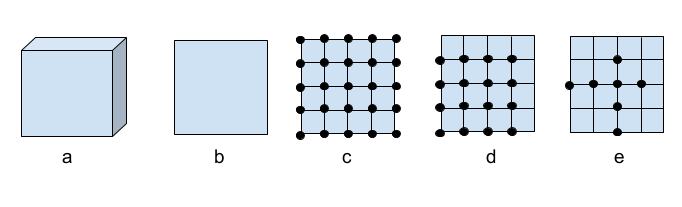
\includegraphics[width=\linewidth]{fig/searchspace.png}
	%\vspace*{-15pt}
	\caption{Reducing the search space}
	\label{fig:searchspace}
\end{figure*}


The main challenge in such methods is to limit the number of trials, since each execution takes up resources and has a monetory cost associated with it. Earlier approaches based on iterative execution have used various techniques such as noisy gradient~\cite{KumarPLPGB16} to converge to a solution faster. In our method, we make use of domain knowledge and heuristics to reduce the search space. Specifically, we employed the following strategies to reduce the parameter space to be explored.

\noindent\subsubsection*{\bf Parameter reduction: }
\label{sec:paramreduction}
The search space is exponential in the number of parameters to be optimized. There are a large number of parameters that can be set for any query. As described in Section~\ref{sec:optmethod}, we have identified a smaller set of parameters that have a relatively larger impact on the performance of sql queries. We restrict the search to these parameters, thus reducing the search space. These parameters have been listed in Tables~\ref{table:job_params}. The search space with a restricted set of parameters is shown in Figure~\ref{fig:searchspace}(a).
\noindent\subsubsection*{\bf Discretization: }
Each parameter, such as memory or partition size, can take a large number of values. However, it can be observed that small changes in the parameters do not have a significant impact. Thus, instead of trying each possible value, it is sufficient to discretize the parameter range and consider only a subset of values for each parameter. These values are placed at a reasonable distance from each other so as to have a significant impact on the query performance. For example, instead of varying memory in units of 1 MB, we can vary it in multiples of 128 MB. The resulting search space is shown in Figure~\ref{fig:searchspace}(b).
\noindent\subsubsection*{\bf Range reduction: }
The range of values for each parameter is further restricted based on domain knowledge about what a good range for that parameter would be.  The knowledge about a good range can be gained by either talking to experts or by looking at some other metrics. For example, for the Hive on MR engine, consider the mapper\_time metric that measures the average time taken by a mapper. If the mapper time is too low, the overhead of starting the mappers is large compared to the actual work done by the mapper. Since the mapper time is inversely related to the number of mappers, the number of mappers need to be reduced. On the other hand, if the mapper time is large, then the job parallelism is restricted and the end to end clock time taken for the query will be high. In this case, more mappers are needed to reduce the work that each mapper has to do. A good acceptable range for this metric could be from 240s till 1800s.  If a set of config params results in mapper\_time beyond the acceptable range, it should not be considered in the search process. For example, mapper\_time is affected by mapreduce.input.fileinputformat.split.maxsize and the correlation is direct, i.e. mapper\_time  increases as we increase mapreduce.input.fileinputformat.split.maxsize.  Thus the split maxsize should be constrained to a range that will lead to a reasonable mapper\_time. In our experiments, we restricted splitsize to between 128 MB and 1 GB. The resulting search space is shown in Figure~\ref{fig:searchspace}(c).
\noindent\subsubsection*{\bf Dimension independence: } 
We make an assumption that the parameters are not correlated to each other. This enables us to optimize each parameter independently of the others. Thus, rather than exploring all the points in the search space, the algorithm explores only one set of values for each parameter as show in Figure~\ref{fig:searchspace}(d). This is a very strong assumption, which may not hold in practice. For example, the mapper memory (mapreduce.map.memory.mb) and the splitsize (mapreduce.input.fileinputformat.split.maxsize) are correlated, since more memory is needed by the mappers as the splitsize increases if spills are to be avoided. Even in this case, the algorithm will find the best value for memory after fixing the splitsize or the best splitsize after fixing the memory. So overall the configuration chosen will be a reasonably good one.

\subsection{Algorithm}
The overall method is listed in Algorithm~\ref{alg:iterativesearch} and is fairly straightforward. It starts with the default value for each configuration parameter (Line 1). It then iterates over the parameters and for each parameter it explores a range of values from low to high, varying it with a minimum step size (Lines 2--6). It runs the query with the chosen parameter values and measures the metric (such as running time or utilization). It finds the value for which the metric is optimized and fixes the value of the parameter to that value before moving on the next parameter (lines 7--12). Finally, it outputs the set of good parameter values $V$ that are discovered in the process.
\renewcommand{\algorithmicrequire}{\textbf{Input:}}
\renewcommand{\algorithmicensure}{\textbf{Output:}}
\renewcommand{\algorithmiccomment}[1]{// #1}
\begin{algorithm}[h]
	\caption{\bf \textit{Iterative Search}}
	\label{alg:iterativesearch}
	\begin{algorithmic}[1]
		%\vspace{1.3em}
		%\small
		\footnotesize
		\REQUIRE Set $\mathcal{P}$ = $\{p_1, p_2 \ldots p_n\}$ of parameters to be determined, the metric $m$ to be optimized, the query $Q$
		\ENSURE The values for parameters in $\mathcal{P}$ that optimize $m$
		\STATE Let $V$ = $\{v_1, v_2, \ldots v_n\}$ = $\{p_1^d, p_2^d, \ldots p_n^d\}$
		\COMMENT {$p_i^l$, $p_i^d$, $p_i^h$ and $p_i^s$ denote the low value, default value, high value and discrete step size for parameter $p_i$}		
		\FOR {Param $p_i$ in $\mathcal{P}$}
			\STATE $m_{best} \gets null$
			\FOR {Value $v$ from $p_i^l$ to $p_i^h$ in steps of $p_i^s$} 
				\STATE Replace $v_i$ by $v$ in $V$
				\STATE Run $Q$ with parameter setting $V$ and measure the metric $m$
				\IF {$m_{best}$ is $null$ or $m$ is better than $m_{best}$}
					\STATE $m_{best} \gets m$
					\STATE $v_{best} \gets v$
				\ENDIF
			\ENDFOR
			\STATE Replace $v_i$ by $v_{best}$ in $V$ \COMMENT{Best value for parameter $p_i$ is found and used in further search}			
		\ENDFOR
		\RETURN $V$
    \end{algorithmic}
\end{algorithm}
  
\subsection{Results}
We evaluated the effectiveness and practicality of the iterative method by running experiments on both synthetic and real workloads. The experiments were carried out for a HIVE on MR engine. The results demonstrated the importance of optimizing the configuration parameters, but at the same time motivated us to explore the model based method instead of the iterative method. We thus present the results here before moving on describing the model based approach.

\subsubsection*{Synthetic Workload}
For synthetic workload, we used the TPC DS dataset (scale 1000) and queries. Each query had to be run a number of times to discover a good set of configuration parameters. To keep the time for the experiments reasonable, we had to use a somewhat small dataset. The average data read by each query was of the order of 20 to 40 GB. The experiments were run on a 4 node cluster on AWS with machine type r3.xlarge. The metric to be optimized was the total resource utilization (Equation~\ref{eqn:totalresource}) and parameters whose values are to be determined are the ones mentioned earlier in Table~\ref{table:job_params}. For each query, we compare the best and worst configuration discovered with the default one in terms of the resource utilization. The results are shown in Figure~\ref{fig:iterativetpcds}. It plots the ratios of the resource usage of minimum to default, maximum to default and maximum to minimum. The min corresponds to the best configuration discovered and max corresponds to the worst configuration among the ones tried out. The graph shows that the min to default ratio varies from 0.18 to 0.73, which indicates that the iterative search leads to a configuration that can save upto 82\% in resource usage over the default configuration. The ratio of max to default is mostly close to 1 and in some cases goes upto 1.80. This indicates that in many cases, the default configuration itself was the worst one (same as max). This is due to the fact that the default split size was 128 MB, leading to a large number of mappers, each processing small amount of data. Since there is some overhead (5-10s) in starting the JVM for each mapper, the startup time becomes significant percentage of the total mapper time if the mapper itself takes very less time to process the data. As a result, the overall query time suffers and resource utilization increases. This suggests that a different default with a larger split size would be more appropriate. Finally, the ratio of max to the min varies from 1.47 to 5.41, indicating that the configuration parameters do make a significant difference in query execution. 
\begin{figure}[h]
	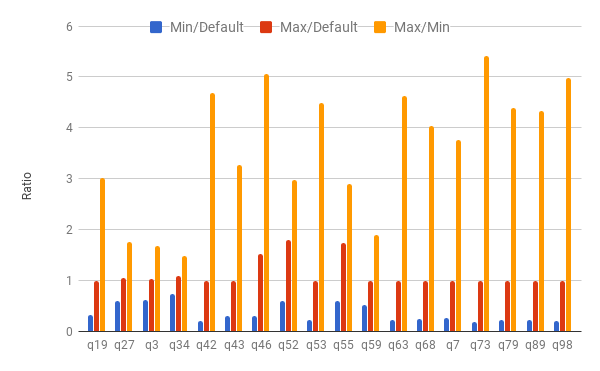
\includegraphics[width=\linewidth]{fig/tpcds-iterative.png}
	%\vspace*{-15pt}
	\caption{Iterative algorithm on TPC DS}
	\label{fig:iterativetpcds}
\end{figure}

\subsubsection*{Real Workloads}
We evaluated the iterative method over real customer data and queries. The workload consisted of three Hive queries running on Hadoop2 MR. These queries were very large and complex and part of their analytics workflow. The input data size was about 400 GB for two of the queries and 200 GB for the third query. The cluster consisted of a r3.2xlarge master node and 30 slave nodes of type r3.8xlarge on AWS Cloud. Figure~\ref{fig:iterativelyft} shows the percentage savings in the total resource utilization cost (Equation~\ref{eqn:totalresource}) of the three queries with the configuration discovered by the iterative algorithm, compared to the cost with the configuration that the customer was using in production. The results show that the iterative algorithm was able to achieve significant savings upto 77\% even for production workloads, indicating that many production workloads are not fully optimized. However, the iterative algorithm took over 50 hours and cost \$5000 since the cluster was quite large with powerful machines. 
\begin{figure}[h]
	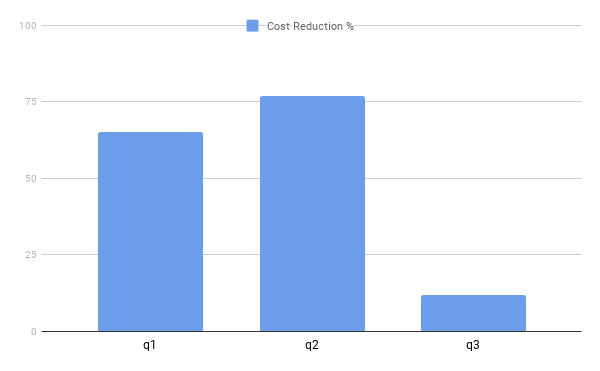
\includegraphics[width=\linewidth]{fig/lyft.png}
	%\vspace*{-15pt}
	\caption{Iterative algorithm on real workload}
	\label{fig:iterativelyft}
\end{figure}

\subsubsection*{Discussion}
The results on synthetic and real datasets show that finding good configuration parameters can lead to significant savings in query costs. The iterative algorithm is able to discover good configuration parameters in a small number of iterations (usually around 10-15 iterations). However, there are some practical limitations as listed below:
\begin{itemize}
	\item The dollar cost of the optimization process can be significant as seen in the real workload. In this case, the customer had 1000 more queries. It may be possible to make the search more efficient and reduce the number of iterations. Since  customers have 100s or 1000s of queries, even 10 or 50 fold reduction is not sufficient to make the approach economical.
	\item For ETL queries, the approach requires shadow clusters and queries. The queries had to be reviewed multiple times to make sure production clusters and tables were not affected. The cost in terms of man-hours is also exorbitant. 	
\end{itemize} 
To address these concerns, we propose a cost model based optimization approach next that does not require multiple executions of the query with different parameters.

\section{Model Based Approach}
\label{sec:modelbased}
We now propose a model for SQL-on-Hadoop engines that builds on the insights described in the previous section. We will describe the model for Apache Hive on Hadoop2 MR and Apache Spark. We will show that even though the model is simple, it is a sufficient approximation to generate good recommendations. 

\subsection{Algorithm}
To model the behavior of a query, we need to know the characteristics of the data processed by the query. This includes the input data size and the output data size for each MR stage of the query processing pipeline. One way to estimate this is to use statistics such as sizes of the tables, number of distinct values for each attribute and histograms that will enable us to estimate selectivities of various operators in the query. However, getting accurate data statistics in a big data environments is very often a challenge. Since we are mainly concerned with ETL queries, we can exploit the fact that these queries are run periodically. SQL-on-Hadoop engines collect a lot of metric and configuration information from the jobs that are executed in the system. The overall approach is thus to use the data collected during a run of the query as inputs to our algorithm to recommend good configuration parameters for future runs of the query. The job metrics and parameters used by the algorithm are listed in Table~\ref{table:job_metrics}. The algorithm also takes as input information about the machine instance type and configuration, as listed in Table~\ref{table:inst_conf}. Besides these, there are some global parameters that can be used to tune the algorithm, as listed in Table \ref{table:global_params}.

\eat{
The inputs to the algorithms are:
\begin{enumerate}
    \item[$\bullet$] Job Parameters: These are the key input parameters of the job that effect performance and cost. Table \ref{table:job_params} defines these job parameters.
    \item[$\bullet$] Instance configuration: Table \ref{table:inst_conf} defines the machine configuration.
    \item[$\bullet$] Global Parameters: These are some of the global parameters that can be used to tune the algorithm. These are defined in Table \ref{table:global_params}.
\end{enumerate}
}

\begin{table}
\begin{tabular}{ |l|p {4.5 cm}| } 
 \hline
 Parameters & Description \\ 
 \hline
 mapperTime  & Total mapper time in seconds   \\ 
 numOfMapper & Number of map tasks \\ 
 mapperMemory & Container memory for map tasks  \\ 
 splitSize & Input Split Size \\
 mapperInputBytes & Map input in bytes \\
 mapperOutputBytes & Map output in bytes \\
 mapperOutputRecords & Number of Map output records \\
 reducerTime & Total reducer time in seconds \\
 numOfReducer & Number of reduce tasks \\
 bytesPerReducer & Corresponds to Hive parameter \textit{hive.exec.reducers.bytes.per.reducer} \\
 reducerMemory & Container memory for reduce tasks \\
 ioSort & Total amount of buffer memory in mega bytes to be used for sorting. Corresponds to Hadoop parameter \textit{mapreduce.task.io.sort.mb} \\
% spilledMapRecords & Number of records spilled in Map tasks  \\
 spilledMapBytes & Bytes spilled in Map tasks  \\
 spilledRedBytes & Bytes spilled in Reduce tasks  \\
 \hline
\end{tabular}
\caption{Job metrics and parameters}
\label{table:job_metrics}
\end{table}

\begin{table}[h]
\begin{tabular}{ |l|p {4.5 cm}| }
 \hline
 Parameters & Description \\ 
 \hline
 nodeMemory  & Total available memory per node for MR job   \\ 
 cpuPerNode & Number of CPUs per node \\ 
 vCpuPerNode & Number of vCPUs per node  \\
 eCPU & computing units per node similar to Amazon ECU \\
 \hline
\end{tabular}
\caption{Instance configuration}
\label{table:inst_conf}
\end{table}

\begin{table}[h]
\begin{tabular}{ |p {1.8 cm}|p {3.5 cm}|p {1 cm} | } 
 \hline
 Parameters & Description & Default\\ 
 \hline
 ioSortFrac & Size of ioSort buffer specified as fraction of mapper memory & 0.4 \\
 maxIOSort & Maximum value for \textit{mapreduce.task.io.sort.mb} & 2047 \\
 reducerFrac & Fraction of Reducer memory to be used as buffer & 0.4 \\ 
 minMapTime & Minimum time that a mapper should take & 60s \\
 minRedTime & Minimum time that a reducer should take & 60s \\ 
 \hline
\end{tabular}
\caption{Global Parameters}
\label{table:global_params}
\end{table}


Algorithm \ref{alg:optres} optimizes cumulative resource utilization of a SQL query. It can be seen from Equation~\ref{eqn:totalresource} that resource utilization can be reduced by decreasing either the memory usage or time taken for processing. The algorithm thus aims to reduce the memory usage without increasing the time. Insight~\ref{insight:mem} indicates that memory usage can reduced without adverse effect by increasing parallelism if necessary. Insight~\ref{insight:parallelism} further says that parallelism should not be increased indiscriminately. Thus the algorithm maintains a lower bound on the mapper and reducer time ($minMapTime$ and $minRedTime$). It first computes the rate of processing of the mappers (line 1), based on the time metric of the previous run and uses it to compute the splitSize, such that each mapper takes at least $minMapTime$ (line 2). It then computes the $ioSort$, such that the output of each mapper fits in that buffer to avoid spills as per Insight~\ref{insight:spill} (line 3--4). The output size of a mapper is estimated using metrics from the previous run (line 3). The mapper memory is computed from the $ioSort$, using the global parameter $ioSortFrac$ (line 5). Similar computations are done to determine the reducer parallelism ($bytesPerReducer$) and $reducerMemory$ (lines 6--9). Finally, the expected resource usage based on the new parameters is computed (line 10--12).

\renewcommand{\algorithmicrequire}{\textbf{Input:}}
\renewcommand{\algorithmicensure}{\textbf{Output:}}
\renewcommand{\algorithmiccomment}[1]{// #1}
\begin{algorithm}
	\caption{OptResource}\label{alg:optres}
	\begin{algorithmic}[1]
		\footnotesize
		\REQUIRE  $\mathcal{P}$ is the job metrics and parameters (defined in table \ref{table:job_params}) from one run, $I$  is instance configuration (defined in Table \ref{table:inst_conf}) on which $\mathcal{P}$ is collected, $\mathcal{G}$ is the global parameters defined in Table \ref{table:global_params}
		\ENSURE New job parameters $\mathcal{P}_{new}$ and the expected cumulative resource usage $expectedResUsage$ after optimization.
		\STATE $mapTimePerByte \gets mapperTime/(mapperInputBytes + spilledMapBytes)$
		\STATE $\mathcal{P}_{new}.splitsize \gets minMapTime/mapTimePerByte$
		\STATE $mapOutPerSplit \gets \mathcal{P}_{new}.splitsize \times (mapperOutputBytes/mapperInputBytes)$
		\STATE $\mathcal{P}_{new}.ioSort \gets mapOutPerSplit$
		\STATE $\mathcal{P}_{new}.mapperMemory \gets \mathcal{P}_{new}.ioSort / ioSortFrac$
		\STATE $redTimePerByte \gets reducerTime/(mapperOutputBytes + spilledRedBytes)$
		\STATE $dataPerRed \gets minRedTime/redTimePerByte$
		\STATE $\mathcal{P}_{new}.bytesPerReducer \gets dataPerRed \times (mapperInputBytes/mapperOutputBytes)$
		\STATE $\mathcal{P}_{new}.reducerMemory \gets dataPerRed / reducerFrac$
		\STATE $numMappers \gets mapperInputBytes/\mathcal{P}_{new}.splitsize$
		\STATE $numReducers \gets mapperInputBytes/\mathcal{P}_{new}.bytesPerReducer$
		\STATE $expectedResUsage \gets numMappers \times minMapTime \times \mathcal{P}_{new}.mapperMemory  + numReducers \times minRedTime \times \mathcal{P}_{new}.reducerMemory$
		\STATE \RETURN $\mathcal{P}_{new}, expectedResUsage$
	\end{algorithmic}
\end{algorithm}



%\begin{algorithm}
%\caption{checkFit} \label{checkfit}
%\begin{algorithmic}[1]
%\footnotesize
%\REQUIRE $\mathcal{P}$ is the job parameters (defined in \ref{table:job_params} ), $\mathcal{I}$  is instance configuration (defined in \ref{table:inst_conf})
%\ENSURE Returns \textit{true} if $\mathcal{P}$ can fit into $\mathcal{I}$, otherwise \textit{false}.
%
%\STATE newMemPerCore $\gets \mathcal{I}.nodeMemory / \mathcal{I}.vCpuPerNode$
%\IF {newMemPerCore $> \mathcal{P}.mapperMemory$ and newMemPerCore $> \mathcal{P}.reducerMemory$}
%\RETURN \textit{true}
%\ELSE
%\RETURN \textit{false}
%\ENDIF
%\end{algorithmic}
%\end{algorithm}

\subsection{Results}
We evaluated the effectiveness of $OptResource$ method by running experiments on real workloads. The experiments were carried out for a HIVE on MR engine for a workload consisting of 4 real customer queries. 
Figure \ref{fig:modelbasedresult} shows the benefit predicted by our model and the actual observed benefit for these queries. The results show that the algorithm leads to significant savings in the cumulative resource usage cost, ranging from 70\% for $q3$ to 90\% for $q2$. Further, the actual savings closely match the predicted savings indicating that the model is reasonably accurate.

\begin{figure}[h]
	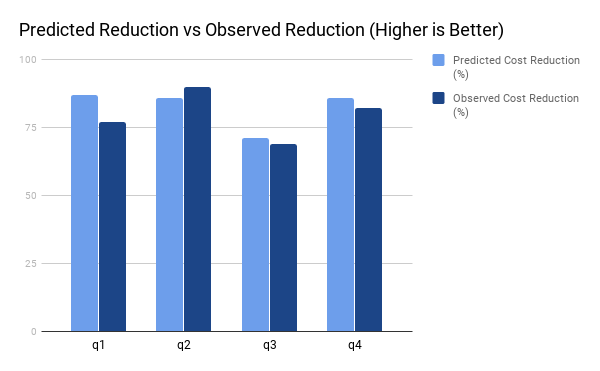
\includegraphics[width=\linewidth]{chart.png}
	%\vspace*{-15pt}
	\caption{Model Based Result: Predicted reduction in cost versus Actual reduction in cost for HIVE on MR queries}
	\label{fig:modelbasedresult}
\end{figure}

We also evaluated effectiveness of the same technique on SparkSQL. Algorithm for it is very similar to $OptResource$ and we are skipping it for brevity. We ran it on 3 real world SparkSQL customer queries. Figure \ref{fig:modelbasedresultspark} shows that the predicted percent reduction in cost matches that of actual reduction is cost observed with very high accuracy.

\begin{figure}[h]
	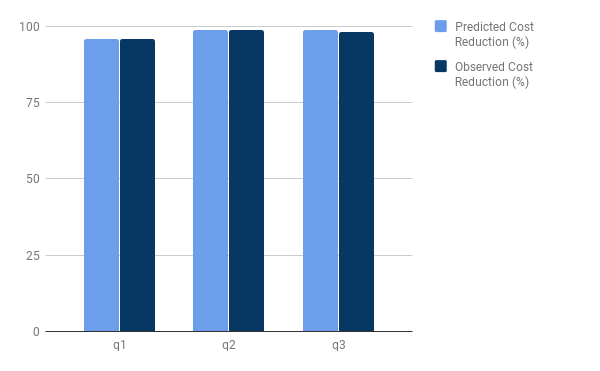
\includegraphics[width=\linewidth]{chart_spark.png}
	%\vspace*{-15pt}
	\caption{Model Based Result: Predicted reduction in cost versus Actual reduction in cost for SparkSQL queries}
	\label{fig:modelbasedresultspark}
\end{figure}
\section{Conclusions}
This paragraph will end the body of this sample document.
Remember that you might still have Acknowledgments or
Appendices; brief samples of these
follow.  There is still the Bibliography to deal with; and
we will make a disclaimer about that here: with the exception
of the reference to the \LaTeX\ book, the citations in
this paper are to articles which have nothing to
do with the present subject and are used as
examples only.
%\end{document}  % This is where a 'short' article might terminate



\appendix
%Appendix A
\section{Headings in Appendices}
The rules about hierarchical headings discussed above for
the body of the article are different in the appendices.
In the \textbf{appendix} environment, the command
\textbf{section} is used to
indicate the start of each Appendix, with alphabetic order
designation (i.e., the first is A, the second B, etc.) and
a title (if you include one).  So, if you need
hierarchical structure
\textit{within} an Appendix, start with \textbf{subsection} as the
highest level. Here is an outline of the body of this
document in Appendix-appropriate form:
\subsection{Introduction}
\subsection{The Body of the Paper}
\subsubsection{Type Changes and  Special Characters}
\subsubsection{Math Equations}
\paragraph{Inline (In-text) Equations}
\paragraph{Display Equations}
\subsubsection{Citations}
\subsubsection{Tables}
\subsubsection{Figures}
\subsubsection{Theorem-like Constructs}
\subsubsection*{A Caveat for the \TeX\ Expert}
\subsection{Conclusions}
\subsection{References}
Generated by bibtex from your \texttt{.bib} file.  Run latex,
then bibtex, then latex twice (to resolve references)
to create the \texttt{.bbl} file.  Insert that \texttt{.bbl}
file into the \texttt{.tex} source file and comment out
the command \texttt{{\char'134}thebibliography}.
% This next section command marks the start of
% Appendix B, and does not continue the present hierarchy
\section{More Help for the Hardy}

Of course, reading the source code is always useful.  The file
\path{acmart.pdf} contains both the user guide and the commented
code.

\begin{acks}
  The authors would like to thank Dr. Yuhua Li for providing the
  matlab code of  the \textit{BEPS} method. 

  The authors would also like to thank the anonymous referees for
  their valuable comments and helpful suggestions. The work is
  supported by the \grantsponsor{GS501100001809}{National Natural
    Science Foundation of
    China}{http://dx.doi.org/10.13039/501100001809} under Grant
  No.:~\grantnum{GS501100001809}{61273304}
  and~\grantnum[http://www.nnsf.cn/youngscientsts]{GS501100001809}{Young
    Scientsts' Support Program}.

\end{acks}

\bibliographystyle{ACM-Reference-Format}
\bibliography{sample-bibliography} 

\end{document}
